\section{Vorstellung}

\begin{frame}[c]{Unifest Allgemein - Design}
    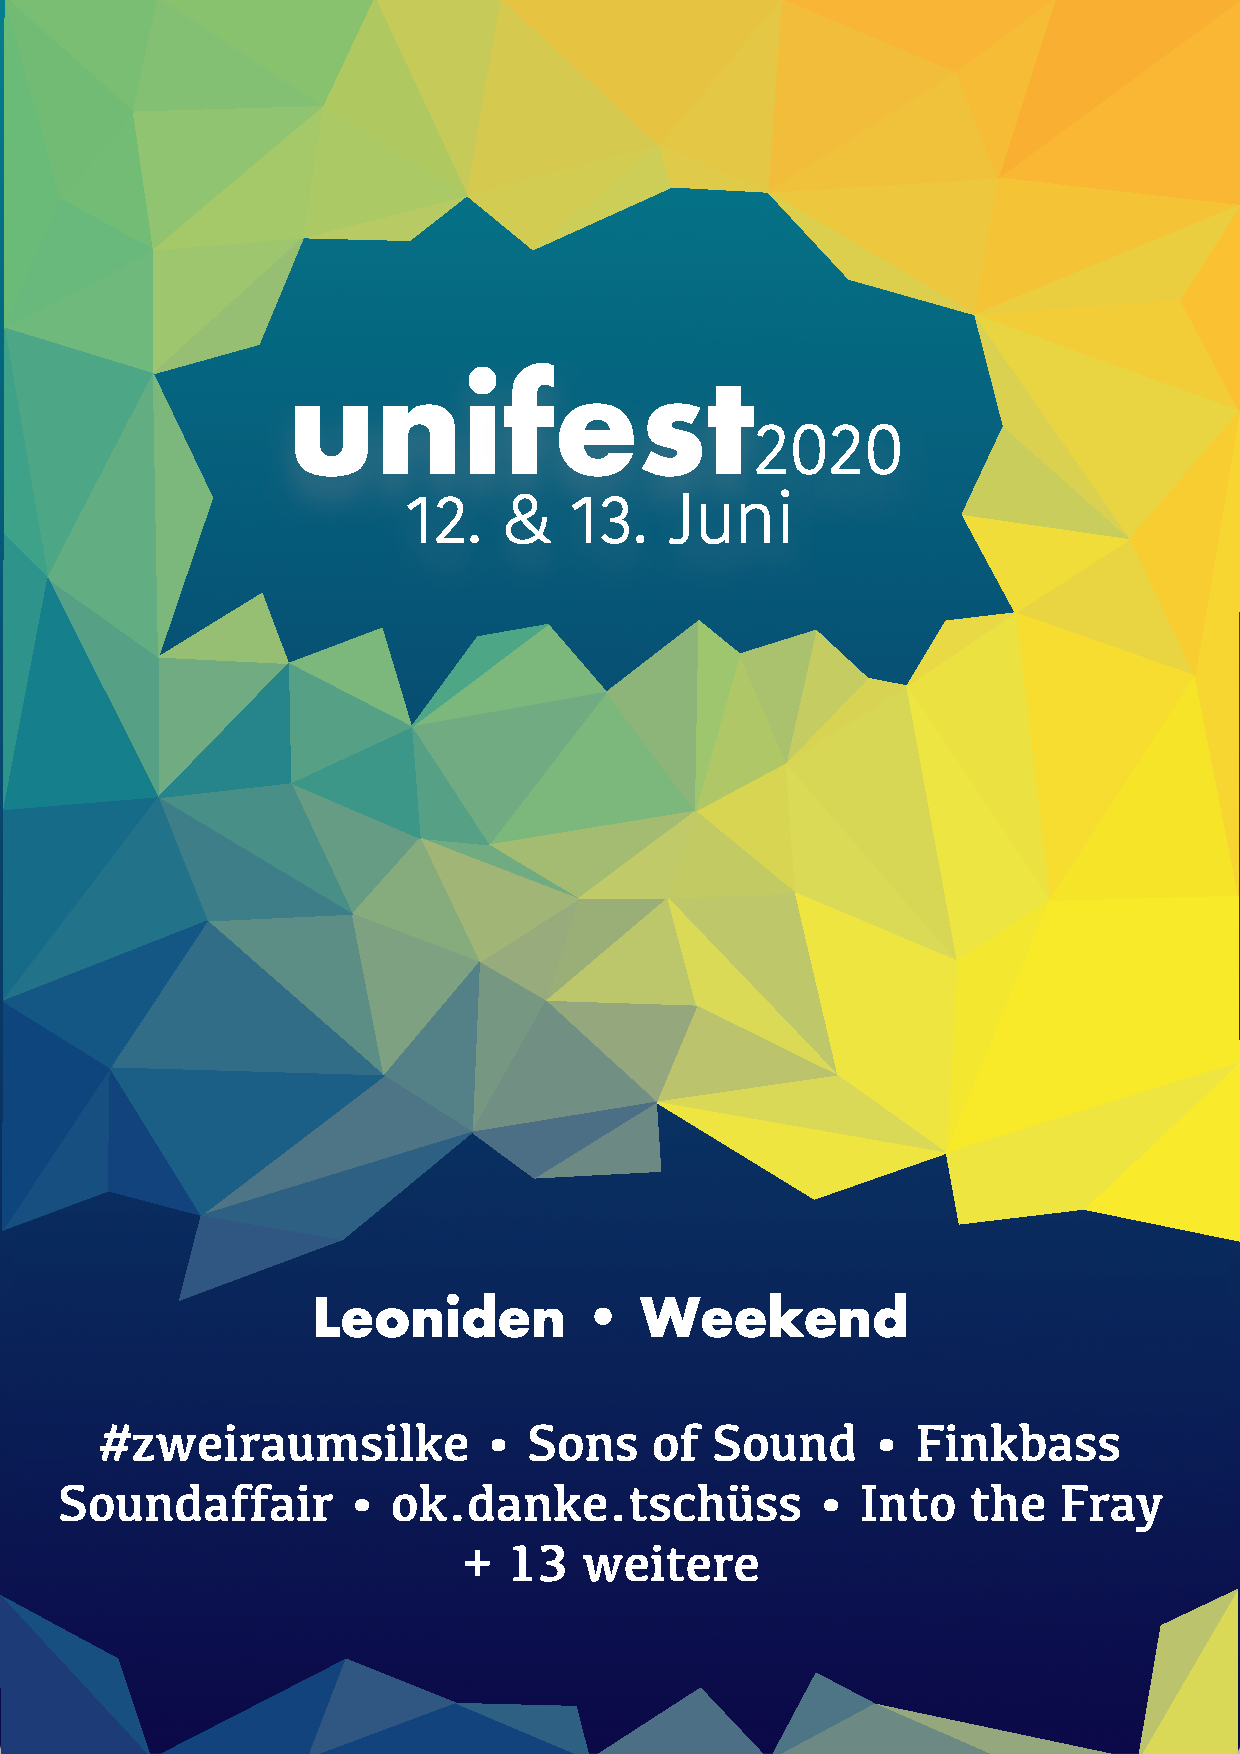
\includegraphics[height=0.8\textheight]{design.pdf} \\
    (Nur Demo-Bands)
\end{frame}


\begin{frame}[c]{Daniela Goth - Vorstellung}
    \begin{itemize}[<+(1)->]
        \item E-Mail: \href{mailto:daniela.goth@asta-kit.de}{daniela.goth@asta-kit.de}
        \item Wirtschaftsingenieurwesen B.Sc. 5. Semester
        \item Vorherige Erfahrung: Helferorga bei Benefizgala
    \end{itemize}
\end{frame}


\begin{frame}[c]{Felix Karg - Vorstellung}
    \begin{itemize}[<+(1)->]
        \item E-Mail: \mailto{fkarg@asta-kit.de}
        \item Informatik M.Sc. 1. Semester
        \item Vorherige Erfahrung: Standbetreuung und Helferorga bei kleineren Events
    \end{itemize}
\end{frame}


\begin{frame}[c]{Festgruppenkoordination - Vorstellung}
    \begin{itemize}[<+(1)->]
        \item E-Mail: \mailto{festgruppenkoordination@unifest-karlsruhe.de}
        \item Teilgruppe der Gesamtkoordination
        \item Mit allen gut vernetzt
        \item Momentane Mitglieder: Felix und Daniela
    \end{itemize}
\end{frame}


\begin{frame}[c]{Festgruppenkoordination - Aufgaben}
    \begin{itemize}[<+(1)->]
        \item Ansprechpartner für alle Festgruppen
        \item Helfersystem-Einführung und Verwaltung (für euch)
        \item Deko-Koordination
        \item Informationsweitergabe an Festgruppen
        \item Festgruppen mit Informationen für Sicherheitskonzepte versorgen
    \end{itemize}
\end{frame}


\begin{frame}[c]{Festgruppenkoordination - Keine Aufgaben}
    \begin{itemize}[<+(1)->]
        \item Ständeaufbaumaterialien: \mailto{material@unifest-karlsruhe.de}
        \item Getränkematerialien: \mailto{bewirtung@unifest-karlsruhe.de}
        \item Allgemeine Helferverwaltung: \mailto{helfen@unifest-karlsruhe.de}
    \end{itemize}
\end{frame}


\begin{frame}[standout]
    Ich möchte einen Stand auf dem Unifest machen. \\
    Wie sieht das Unifest dieses Jahr aus?
\end{frame}


\section{Festkonzept}

\subsection{Allgemein}

\begin{frame}[c]{Übersicht Festkonzept}
    \begin{itemize}[<+(1)->]
        \item Keine Floors
        \item Drei Hauptbühnen:
            \begin{itemize}[<+(1)->]
                \item Forum
                \item Otto-Amann-Platz
                \item Paulckeplatz
            \end{itemize}
        \item Umzäuntes Gelände, Tickets für 5\EUR/Tag
        % \item (Aufbau-) Helfer bekommen Tickets erstattet (für den Tag an dem sie Helfen)
        \item Helfer bekommen gratis Eintritt für den Tag an dem sie Helfen
    \end{itemize}
\end{frame}



\subsection{Stände}

\begin{frame}[standout]
    Wo kann ich meinen Stand hinstellen?
\end{frame}


\begin{frame}[c]{Standplatzierung}
                                    % trim = left bottom right top
    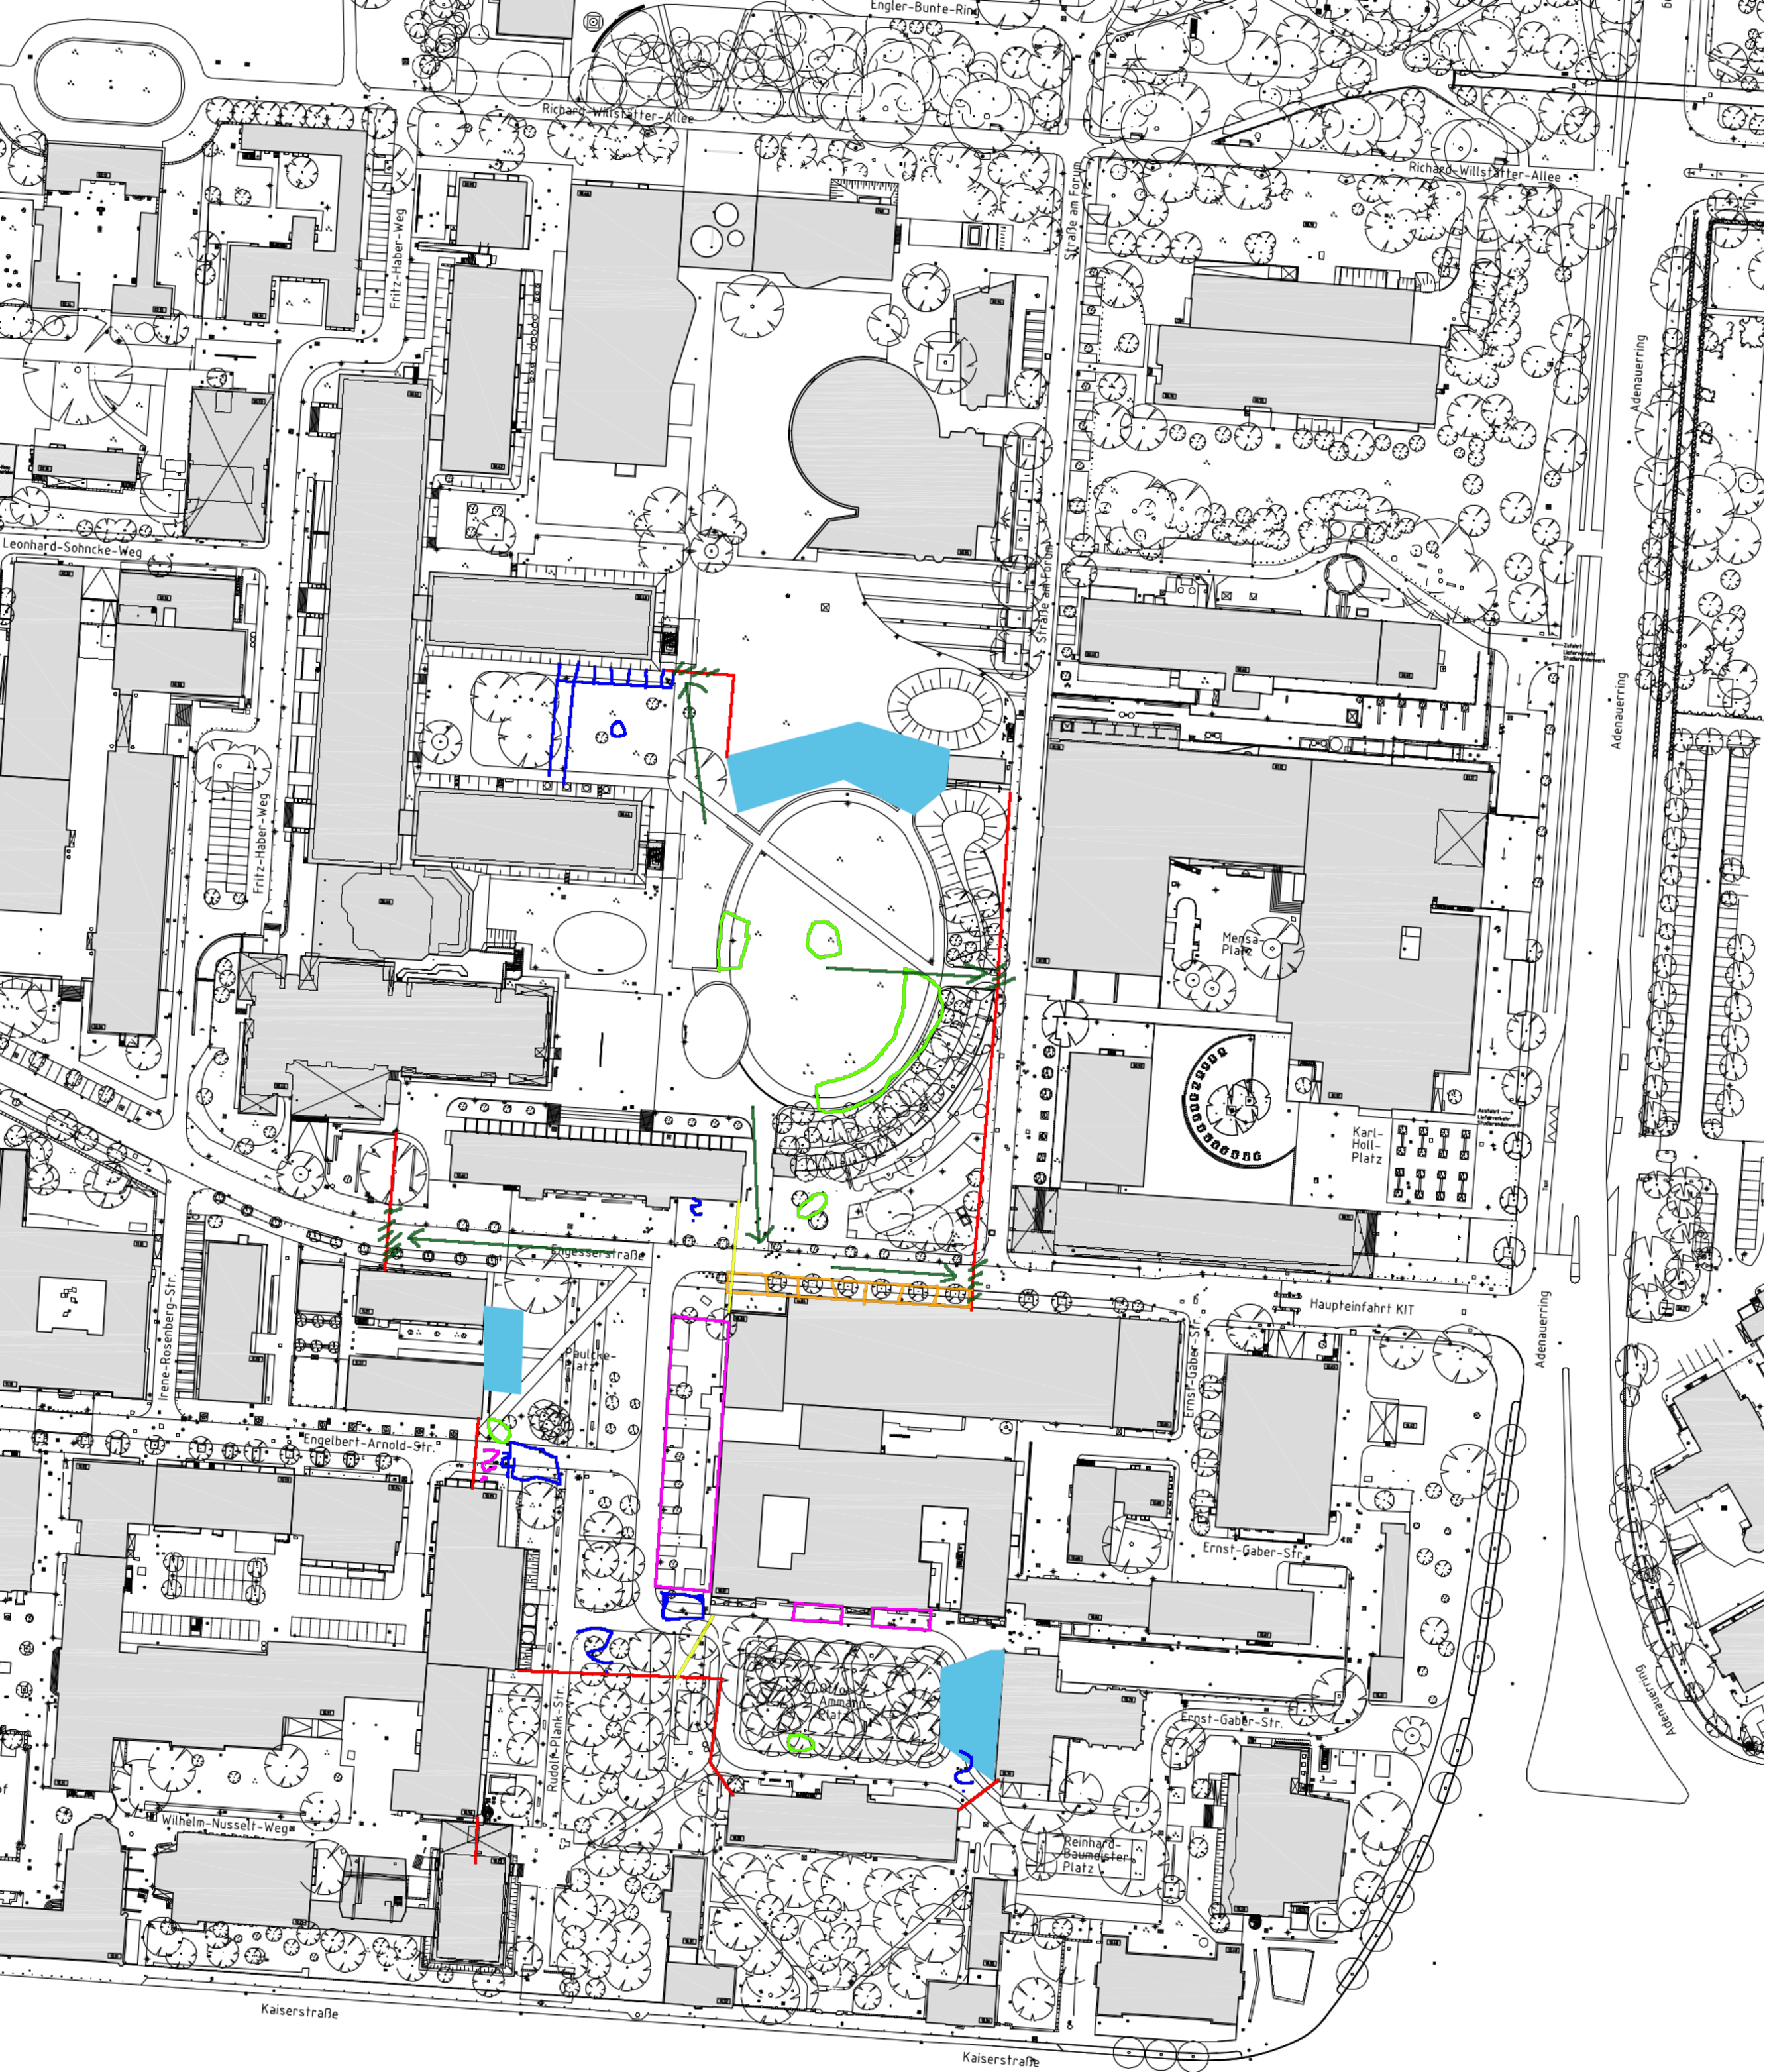
\includegraphics[height=\textheight,clip,trim = 200 20 0 400]{PlanSketch.pdf} \\
    \pnote{Sagen: Bei Forum nur Manpower stellen, man kann dafür eventuell ein Banner an den stand hängen}
    \pnote{Jan um neueres Bild bitten}
\end{frame}



\begin{frame}[standout]
    Kann ich meinen Stand frei gestalten?
\end{frame}

\begin{frame}[c]{Standgestaltung}
    \begin{itemize}[<+(1)->]
        \item Ja, ihr könnt euren Stand frei gestalten!
        \item Es gibt ein Stand-Design-\textbf{Vorschlag}
        \item Allerdings könnt ihr da alles für euch optimieren!
        \item Platziert eure Banner wie ihr wollt!
        \item Alles was 'realistisch' ist, könnt ihr bei uns anfragen!
        \item Es gibt Budget für Deko: Ihr könnt mit Ideen auf uns zukommen!
        \item Details können mit uns abgesprochen werden
    \end{itemize}
\end{frame}


\begin{frame}[standout]
    Was kann ich an meinem Stand anbieten?
\end{frame}

\begin{frame}[c]{Standangebote}
    \begin{itemize}[<+(1)->]
        \item Idealerweise etwas zu Trinken
        \item Kein Bier (es gibt genug Bierinseln)
        \item Keine Longdrinks (!)
        \item Muss nicht Alkfrei sein (Bieten Bierinseln an)
        \item Idealerweise: Ein Fancy Cocktail (gerne in Variation)
        \item Oder: Mehrere Shots
        \item Oder: Met, Wein-Whisky, ...
    \end{itemize}
\end{frame}


\begin{frame}[standout]
    \pnote{Alles in 0.4L Bechern/Gläsern}
    Kann ich auch einen Stand nur mit Manpower besetzen?
\end{frame}

\begin{frame}[c]{Nur Manpower stellen}
    \begin{itemize}[<+(1)->]
        \item Ja, man kann dann z.B. die Bierinseln bedienen
        \item Oder die Cocktailstände im Forum
        \item Dafür kann man dann auch sein Banner dort aufhängen
        \item (Allerdings bekommt ihr dann nichts vom Standgewinn)
    \end{itemize}
\end{frame}

\begin{frame}[standout]
    Von wann bis wann müssen die Stände besetzt werden?
\end{frame}

\begin{frame}[c]{Standbesetzung}
    \begin{itemize}[<+(1)->]
        \item Ausschank-ende ist für alle Mitternacht
        \item Anfangen dürft ihr wann ihr wollt - die meisten werden Mittags noch keinen Cocktail wollen
    \end{itemize}
\end{frame}

\subsection{Finanzierung}

\begin{frame}[standout]
    Werden wir am Gewinn vom Unifest beteiligt?
\end{frame}


\begin{frame}[c]{Gewinnbeteiligung}
    \begin{itemize}[<+(1)->]
        \item Ja, Ihr werdet am Gewinn beteiligt!
        \item Proportional zu geleisteten Helferstunden, nicht Standgewinn!
        \item Abgezogen wird: Überdurchschnittlicher Schankverlust eures Standes :)
    \end{itemize}
\end{frame}


\begin{frame}[standout]
    Welche Kosten kommen auf uns zu?
\end{frame}

\begin{frame}[c]{Finanzierung und Gewinn}
    \begin{itemize}[<+(1)->]
        \item Wissen wir noch nicht.
        \item Momentan als Konzept: Zwei Modelle
        \item Variante Eins: Standgebühr und (Umsatz-) Freibetrag
        \item Variante Zwei: Direkt Prozentualer Gewinn
        \item Eigentliche Gewinnbeteiligung: Proportional zu Helferarbeit
        \item Was denkt ihr darüber?
    \end{itemize}
\end{frame}


\begin{frame}[c]{Kosten die nicht auf euch zukommen}
    \begin{itemize}[<+(1)->]
        \item Zusätzlich Kosten für Standmaterialien (wenn dann eine fixe Standgebühr)
        \item Kosten für eure Zubereitungsmaterialien
        \item Kosten für Strom oder Wasser (Strom zahlt das KIT)
    \end{itemize}
\end{frame}



\subsection{Helfen}

\begin{frame}[standout]
    Wie kann ich beim Unifest mithelfen?
\end{frame}


\begin{frame}[c]{Helfen beim Unifest}
    \begin{itemize}[<+(1)->]
        \item Im Helfersystem anmelden und für Aufgaben freischalten lassen
        \item Wir werden dieses Jahr ein anderes Helfersystem verwenden
        \item Eure Stände (und Schichten) werden auch über das Helfersystem abgebildet
        \item Es gibt auch noch viele weitere Helferschichten
        \item Wir machen kurz vor dem Unifest eine Einführung in das Helfersystem
    \end{itemize}
\end{frame}


\section{Nächstes Treffen}

\begin{frame}[c]{Nächstes Treffen}
    \begin{itemize}[<+(1)->]
        \item Ungefähr Ende Februar
        \item Vermutlich wieder Hier
        \item Idealerweise: Ihr habt Ideen was ihr tun wollt
        \item Z.B.: Was für einen Cocktail
        \item Z.B.: Wie groß der Stand sein soll
        \item Z.B.: Wie euer Stand grob aussehen soll
    \end{itemize}
\end{frame}


\begin{frame}[c]{Zukünftige Kommunikation}
    Mailverteiler:
     \begin{itemize}[<+(1)->]
         \item Bitte uns Mailadresse mitteilen!
     \end{itemize}

     \pause
     Telegram-Gruppe:
    \begin{itemize}[<+(1)->]
        \item Wir werden eine Standbetreuer-Telegram-Gruppe erstellen, vor allem für das Fest selbst interessant
    \end{itemize}
\end{frame}



